\subsection{Assigning frequencies/channels to radiostations/mobile phone base stations}

If you put base stations (towers) too close, they must not interfere with each other.
Hence, they must work on different frequencies.
This is where graph coloring is used.
An each distinctive color will represent each distinctive frequency.

Represent towers as vertices.
If towers are placed too close to each other, put an edge between them, meaning, different colors/frequencies must be assigned to them.

For cellular network, placing stations/tower in hexagonal form, makes this graph to be colored using only 3 colors/frequencies:

\begin{figure}[H]
\centering
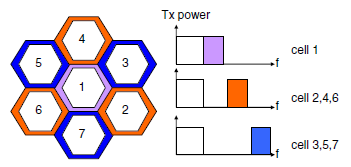
\includegraphics[scale=0.85]{color/freq.png}
\caption{Example}
\end{figure}

( The images was taken from the 
\href{https://jwcn-eurasipjournals.springeropen.com/articles/10.1186/1687-1499-2012-230}{Generalizing and optimizing fractional frequency reuse in broadband cellular radio access networks} article. )

Mathematicians say, the chromatic number of this (planar) graph is 3.
Chromatic number is a minimal number of colors.
And a planar graph is a graph that can be represented on 2D plane with no edges intersected (like a world map).

See also: \url{https://en.wikipedia.org/wiki/Radio_coloring}.

